% -------------------------------------------------------
% Bug: Unrecognized Opcode
% -------------------------------------------------------
\section{Challenge 2 Level 1 (C2L1): Unrecognized Opcode}

This Section presents the tool Automated Assembly Program Generator as well as the bug description and solution proposed.

\subsection{Automated Assembly Program Generator (AAPG)}

The \texttt{aapg} is a versatile tool used to automatically generate assembly programs for RISC-V architectures based on specified configurations. It simplifies the process of creating complex assembly programs, especially when testing and evaluating RISC-V processors or architecture extensions. By defining various parameters and characteristics in a configuration file, users can customize the generated assembly code to suit their specific use cases.

The \texttt{aapg} supports a wide range of RISC-V extensions, allowing users to include or exclude specific instructions and features as needed. It also provides options to control the level of complexity in the generated code, such as the number of instructions, branching patterns, and data dependencies.

With the \texttt{aapg} tool, users can quickly create diverse assembly programs for testing processor functionalities, evaluating performance, and verifying hardware implementations.

\subsection{Bug}

In the context of using the \texttt{aapg} tool, a bug has been encountered, resulting in ``unrecognized opcode" errors during the assembly process.

The provided config file ``rv32i.yaml" is used to configure the desired extension and other characteristics of the design. This configuration file instructs the \texttt{aapg} to generate assembly code that adheres to the RV32I base integer instruction set, which includes the standard integer arithmetic, logical, and control flow instructions.

However, in the current context, the bug has occurred due to the inadvertent addition of RV64M instructions. The RV64M extension includes instructions that are not part of the RV32I base instruction set. As a result, when the \texttt{aapg} generates assembly code with these additional RV64M instructions, the assembler encounters errors of the type "Error: unrecognized opcode." This happens because the assembler cannot recognize and process the non-supported RV64M instructions while attempting to assemble the code intended for RV32I.

\subsection{Solution}

To resolve this bug, it is necessary to update (turn off) the generation of RV64M instructions. To do this, change the code according with Figure \ref{fig:rv32i_diff}. 


\begin{figure}[H]
    \centering
    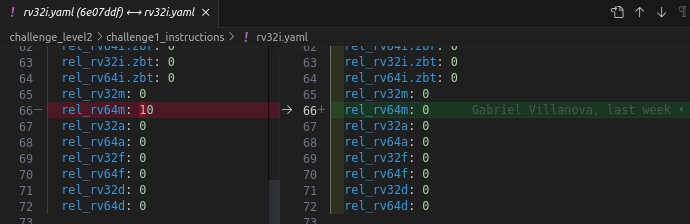
\includegraphics[width=0.48\textwidth]{./rv32i_diff.png}
    \caption{Updated code for AAPG generation in C2L1 bug.}
    \label{fig:rv32i_diff}
\end{figure}


By making this modification, the \texttt{aapg} will no longer generate RV64M instructions, ensuring that the assembler doesn't encounter any ``unrecognized opcode" errors as is shown in Figure \label{ref:unrec}.

\begin{figure}[H]
    \centering
    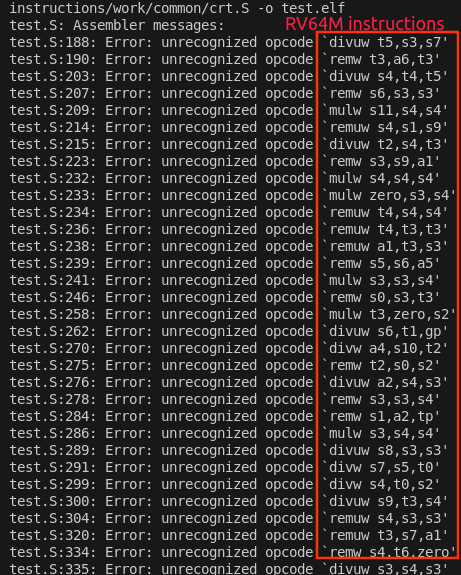
\includegraphics[width=0.48\textwidth]{./unrec_op.png}
    \caption{Unrecognized instruction error due to RV64M generation in AAPG.}
    \label{fig:unrec}
\end{figure}
